\documentclass[a4paper]{article}
\usepackage{preamble}

% Setup title
\title{MATHEMATICS 2 - TERM 2}
\author{Marc Sanchis}
\date{April 2024 - June 2024}

\begin{document}

% Title
\newgeometry{top=2cm, bottom=5.5cm}
\maketitle

% Table of Contents
\renewcommand{\contentsname}{}
\tableofcontents

% Body
\newpage
\restoregeometry
\pagestyle{fancy}
\setcounter{section}{5}

\section{Introduction to Differential Equations}

A differential equation (DE) is an equation containing one or more dependent variable derivatives, like \textit{Newton's Law}
$$
F=m \frac{d^{2}x(t)}{dt^{2}}=mx''=m\ddot{x}
$$

DEs with one independent variable are called \textbf{Ordinary Differential Equations} (ODE); an example can be the \textit{Radioactive Disintegration} $m'=km$, where $k$ is an independent variable.

DEs with multiple independent variables and partial derivatives are called \textbf{Partial Differential Equations}; an example can be the \textit{Wave Equation}
$$
\nabla u\equiv\nabla^{2}u=\frac{\partial^{2}u(\mathbf{x}, t)}{\partial x^{2}}+\frac{\partial^{2}u(\mathbf{x},t)}{\partial y^{2}}+\frac{\partial^{2}u(\mathbf{x},t)}{\partial z^{2}}=\frac{1}{c^{2}}\frac{\partial^{2}u(\mathbf{x},t)}{\partial t^{2}}
$$

\vspace{1ex}\note{The largest order of derivative defines the order of the DE. An ODE is lineal for $F(t,y,y',\dots,y(n))=0$}\vspace{1ex}

An ODE can be solved with a general ($=\dots+C$) or particular ($=\dots+k,\,k=\mathbb{R}$). The result can be given by an Initial Value Problem (IVP): a function $f(t)$ verifying the ODE and the Initial Condition (IC).

\vspace{1ex}\note{Frontier problems are an IVP but verifying an IC relative to the contour, a Contour Condition (CC)}\vspace{1ex}

\section{First Order Differential Equations}

\subsection{Separable DE}
A first-order ODE $F(t,y,y')$ is \textit{separable} if it can be written as
$$
A(t)dt=B(y)dy,\hspace{4ex}y'=\frac{A(t)}{B(y)},\hspace{4ex}y'=C(t)D(y)
$$

\vspace{2ex}\textit{\textbf{Prob.:}} A bowl filled with water spins at a $w$ velocity. If we put a mass $m$ on the surface of the water and denote tension force by $T$, centrifugal force by $F_{c}$ and weight by $P$. Formulate Newton's Equation.

\begin{align}
F&=ma, & v&=cte\implies a=0 \\
F&=0, & \sum^{}_{}F&=P+F_{c}+T \\
0&= P+F_{c}+T
\end{align}
$$
P=-mg\mathbf{j},\, F_{c}=mR\omega 2i,\, T=-T\sin \alpha \mathbf{i} + T\cos \alpha \mathbf{j}
$$
Where $T=\mid\mid \mathbf{T}\mid\mid$ and $\alpha$ is the angle between the tangent and the horizontal axis

\begin{minipage}{0.4\textwidth}
equalling these terms
\begin{align}
\begin{cases}
T\sin \alpha=mR\omega^{2}, \\
T\cos \alpha=mg
\end{cases} \\
R\omega^{2}g=\tan \alpha
\end{align}
$$
\boxed{\frac{\omega^{2}}{g}x=\frac{dy}{dx}}
$$
\end{minipage} \hfill \begin{minipage}{0.4\linewidth}
\begin{figure}[H]
    \centering
    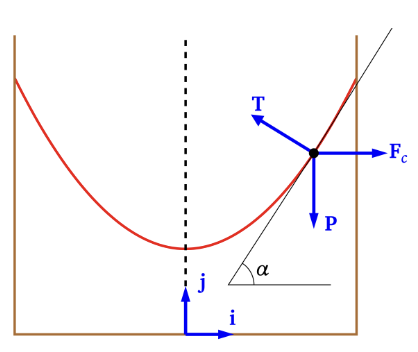
\includegraphics[width=\textwidth]{IMG/ex_water.png}
    \caption{Water bowl example}
    \label{fig:ex_water}
\end{figure}
\end{minipage}



\subsection{Homogeneous ODE}

\vspace{1ex}\note{A function $f(x,y)$ is said to be of order $n$ if $f(\lambda x,\lambda y)=\lambda^nf(x,y)$}\vspace{1ex}

A first-order ODE $M(x,y)dx+N(x,y)dy=0$ is homogeneous if and only if $M$ and $N$ are of the same order.

\vspace{1ex}\note{Given a homogeneous ODE $dy / dt=f(t,y)$, it can be solved by making the change $u=y / t$ converting the equation into a separable variables equation}\vspace{1ex}

\vspace{2ex}\textit{\textbf{Ex.:}} $t^{3}y'=t^{2}y-2y^{3}$
\begin{align} 
y'=\frac{t^{2}y-2y^{3}}{t^{3}}&=\frac{y}{t}-2\left( \frac{y}{t} \right)^{3} \\
u&=y / t \\
f(y / t)&=f(u)=u-2u^{3} \\
y'=\frac{dy}{dt}&=\frac{d(ut)}{dt}=\frac{du}{dt}t+u \\
\frac{du}{dt}t+u&=u-2u^{3} \\
\frac{du}{2u^{3}}&=-\frac{dt}{t}
\end{align}

\vspace{2ex}\textit{\textbf{Prob.:}} Find the form of a curved mirror that divides a beam of light parallel to the $X$ axis.

The beams will be reflected towards a point we will be calling $F$ (property of a parabolic antenna).

\begin{figure}[H]
    \centering
    \begin{subfigure}{0.3\textwidth}
        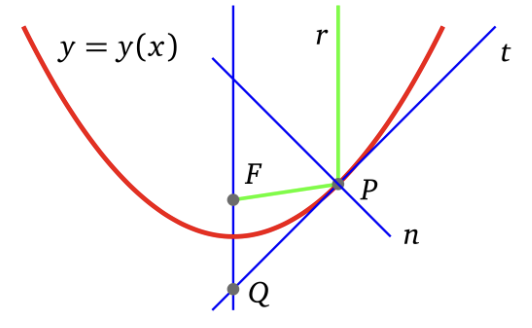
\includegraphics[width=\textwidth]{IMG/prob_mirror1.png}
    \end{subfigure}\hspace{5ex}
    \begin{subfigure}{0.3\textwidth}
        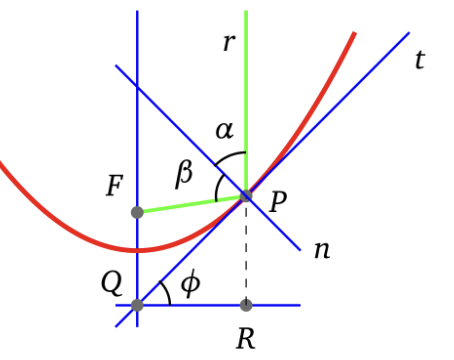
\includegraphics[width=\textwidth]{IMG/prob_mirror2.png}
    \end{subfigure}
    \caption{Parabolic mirror problem}
    \label{fig:prob_mirror}
\end{figure}

Let the axis through $\overline{FQ}$ be $y$, $P(x,y)$ is the intersection of the beam and the mirror, $t$ being its tangent and $n=\mid\mid t\times y(x)\mid\mid$ the normal. The angles denoted by $\alpha,\beta,\phi$. For $r \perp x \implies \phi=\alpha$, and following \textit{Snell's Law} $\alpha=\beta$, and by geometry $\alpha=\phi$, so $\alpha=\beta=\phi$. Knowing this, we can affirm that the triangle formed by $PQF$ is isosceles, implying $PF=FQ$.

$\phi=dy / dx=\frac{PR}{QR}$ and if we place $F$ on $(0,0)$, then $PR=y+FQ=y+\sqrt{ x^{2}+y^{2} }$ and $QR=x$, so
$$
\frac{dy}{dx}=\frac{y+\sqrt{ x^{2}+y^{2} }}{x}\hspace{4ex}\leftarrow\text{homogeneous}
$$
and we can make $u=y / x$
\begin{align}
\frac{d(ux)}{dx}&=\frac{ux+\sqrt{ x^{2}+(ux)^{2} }}{x}\implies \\
\implies&u+x \frac{du}{dx}=u+\sqrt{ 1+u^{2} }\implies \\
\implies&x \frac{du}{dx}=\sqrt{ 1+u^{2} } \implies
\end{align}
$$
\boxed{\frac{du}{\sqrt{ 1+u^{2} }}=\frac{dx}{x} \implies F(y / x)=\log x+C}
$$

\vspace{2ex}\textit{\textbf{Ex.:}} Solve for $y'=(2y-t+1) / (t+y+3)$
\begin{align}
f(\lambda y,\lambda t)&=\frac{2\lambda y-\lambda t+1}{\lambda y+\lambda t+3}, & &\leftarrow\text{not homogeneous}
\end{align}
$$
y=Y+a,\hspace{4ex}t=T+b,\hspace{4ex}a,b=\mathbb{R}
$$
\begin{align}
\frac{dY}{dT}&=\frac{2(Y+a)-(T+b)+1}{(Y+a)+(T+b)+3}= \\
&= \frac{2Y-T+(2a-b+1)}{Y+T+(b+a+3)}
\end{align}

For the equation to be homogeneous, we must solve
$$
\begin{cases}
2a-b+1=0, \\
b+a+3=0
\end{cases}\implies \begin{cases}
a=-4 / 3, \\
b=-5 / 3
\end{cases}
$$
$$
\boxed{\frac{dY}{dT}=\frac{2Y-T}{Y+T}}\hspace{4ex}\leftarrow\text{homogeneous}
$$

\vspace{2ex}\textit{\textbf{Prob.:}} Solve the equation above \textbf{TODO}

\vspace{2ex}\textit{\textbf{Ex.:}} Solve for $y'=(2y-t+1) / (y+t+3)$
\begin{align}
f(\lambda y,\lambda t)&=\frac{2\lambda y-\lambda t+1}{\lambda y+\lambda t+3}\hspace{4ex}\leftarrow\text{not homogeneous} \\
y'=\frac{dy}{dt}&=\left\langle\begin{cases}
2y+6t=1, \\
3y+9t=0
\end{cases}\right\rangle =\frac{2(y+3t)-1}{3(y+3t)} \hspace{4ex}\leftarrow\text{parallel functions}
\end{align}

As the functions are parallel, the previous method will not work, but we can make a variable change $u=y+3t$
$$
\boxed{\frac{du-3\,dt}{dt}=\frac{2u-1}{3u}}
$$
\vspace{2ex}\textit{\textbf{Prob.:}} Solve the above equation

\subsection{Exact DEs}
An $M(t,y)dt+N(t,y)dy=0$ DOE is \textit{exact} if its \textit{potential function} $F(t,y)$ exists as
$$
\frac{\partial F}{\partial t}=M(t,y),\hspace{4ex} \frac{\partial F}{\partial y}=N(t,y)
$$
for an \textit{exact DOE} 
$$
F(t,y)=\text{const}
$$

To prove this on any equation of this style
$$
\frac{\partial M}{\partial y}=\frac{\partial N}{\partial t}
$$
\vspace{2ex}\textbf{\textit{Ex.: }}Solve $(2ty+3t^{2}y^{2}+1)dt+(t^{2}+2t^{3}y+2y)dy=0$ 
$\triangleright$ Define $M(y,t)=2ty+3t^{2}y^{2}+1$ and $N(y,t)=t^{2}+2t^{3}+2y$ and observe
$$
\partial_{t}F=2t+6t^{2}y=\partial_{y}N\hspace{4ex}\leftarrow\text{Exact DOE}
$$
$\triangleright$ Find $F(y,t)$
\begin{align}
\text{Exact DOE}\implies \partial _{t}F&=M(y,t)=2ty+3t^{2}y^{2}+1 \\
\partial_{y}F&=N(y,t)=t^{2}+2t^{3}y+2y
\end{align}
$\triangleright$ Integrate
\begin{align}
F(y,t)=\int (2ty+3t^{2}y^{2}+1) \, dt\, =yt^{2}+t^{3}y^{2}+t+g(y)
\end{align}
$\triangleright$ Determine $g(y)$
\begin{align}
\partial_{y}F=t^{2}+2t^{3}y+\frac{dg}{dy}&=N(y,t)=t^{2}+2t^{3}y+2y \\
\frac{dg}{dy}&=2y \\
g(y)&=y^{2}+C \\
\end{align}
$\triangleright$ Solve with $g(y)$
\begin{align}
F(y,t)=yt^{2}+t^{3}y^{2}+t+y^{2}+C=K'
\end{align}
$$
\boxed{K=yt^{2}+t^{3}y^{2}+t+y^{2}}
$$
\vspace{2ex}\textbf{\textit{Prob.: }}Solve (using $N$) $(3y+2)dt+(8t+8y)dy=0$
$\triangleright$ $M(y,t)$ and $N(y,t)$ already defined, find $F(y,t)$ 
\begin{align}
\text{Exact DOE}\implies \partial_{y}F(y,t)&=N(y,t) \\
F(y,t)&=\int (3t+8y) \, dy\, =3ty+4y^{2}+g(t)
\end{align}
$\triangleright$ Determine $g(t)$
\begin{align}
\partial_{t}F(y,t)=3y+&0+\frac{dg}{dt}=3y+2 \\
g(t)&=2t+C
\end{align}
$\triangleright$ Solve with $g(t)$ 
\begin{align}
F(y,t)=3ty+4y^{2}+2t+C=K'
\end{align}
$$
\boxed{K=3ty+4y^{2}+2t}
$$
\subsection{Integral Factor}
\textbf{\textit{Read Integral Factor (point 5)}}

\subsection{Lineal Equations}
A Lineal Equation (LE) is defined by a DE expressible as $y'+p(t)y=q(t)$. To solve a Lineal Ordinal Differential Equation (LODE), it is multiplied by $\mu=e^{ \int p(t) \, dt\, }$  and try to get the derivative of a product with $\mu'$ in function of $\mu$ on the other side, like so
$$
\mu'=D_{t}\mu=e^{ \int p(t) \, dt\,  }p(t)=\mu p
$$
\begin{align}
\mu y'+\mu py=\mu p\implies \mu y'+\mu'y=\mu q\implies(\mu y)'=\mu q
\end{align}
then the expression can be integrated
\begin{align}
\mu y=\int \mu q \, dt\, \implies
\end{align}
$$
\boxed{y=\frac{1}{\mu}\int \mu q \, dt\, }
$$
\vspace{1ex}\note{$\mu$ is a function of $t$ and can not be moved in or out of the integral}\vspace{1ex}

\vspace{2ex}\textbf{\textit{Ex.: }}Solve $y'+2y=e^{t}$
$\triangleright$ Determine linearity and define $p(t)$ and $q(t)$
$$
\text{Linear}\implies p(t)=2,\hspace{4ex}q(t)=e^{ t }
$$
$\triangleright$ Find $\mu=e^{ \int p(t) \, dt\, }$
\begin{align}
\int p(t) \, dt\, =\int 2 \, dt\, =2t\implies \mu=e^{ 2t }
\end{align}
$\triangleright$ $\mu'$ in function of $\mu$
\begin{align}
\mu'=2\mu
\end{align}
$\triangleright$ Multiply by $\mu$ and obtain the derivative on the other side
\begin{align}
\mu y'+\mu 2y=\mu e^{ t }\implies(\mu y)'=\mu e^{ t }
\end{align}
$\triangleright$ Solve by obtaining $y$
\begin{align}
\mu y=\int \mu e^{ t } \, dt\, &=\int e^{ 2t }e^{ t } \, dt\, =\int e^{ 3t } \, dt\, =\frac{e^{ 3t }}{3}+C \\
y&=\frac{1}{e^{ 2t }}\left( \frac{e^{ 3t }}{3}+C \right)
\end{align}
$$
\boxed{y=\frac{e^{ t }}{3}+C\,e^{ -2t }}
$$

\vspace{2ex}\textbf{\textit{Prob.: }}Solve $(y+x^{2}\cos x)dx-xdy=0$ 
$\triangleright$ Define $M(x,y)=y+x^{2}\cos x$ and $N(x,y)=-x$
$$
D_{y}M(x,y)=1,\hspace{4ex}D_{x}N(x,y)=-1 \hspace{4ex}\leftarrow\text{Not exact DOE}
$$
$\triangleright$ Determine linearity and find $p(x)$ and $q(x)$
\begin{align}
(y+x^{2}\cos x)+xy'&=0 \\
(y+x^{2}\cos x)&=xy' \\
\left( \frac{y}{x}+x\cos x \right)&=y' \\
y'-\frac{y}{x}=x\cos x
\end{align}
$$
p(x)=-\frac{1}{x},\hspace{4ex}q(x)=x\cos x
$$
$\triangleright$ Find $\mu$
\begin{align}
\int p(x) \, dx\, &=\int -\frac{1}{x} \, dx\, =-\log x \\
\mu&=e^{ -\log x }=\frac{1}{x}
\end{align}
$\triangleright$ Express $\mu'$ in function of $\mu$
\begin{align}
\mu'=-\frac{\mu}{x}
\end{align}
$\triangleright$ Multiply by $\mu$ and find the derivative on the other side
\begin{align}
\mu y'+\frac{\mu y}{x}=\mu x\cos x \implies (\mu y)'=\cos x
\end{align}
$\triangleright$ Solve by obtaining $y$
\begin{align}
\mu y&=\int \cos x \, dx\, =\sin x+C  \\
y(x)&=\mu^{-1}\sin x+C
\end{align}
$$
\boxed{y(x)=x(\sin x+C)}
$$
\subsection{Curve Family}
An expression $F(x,y,K)=0,\,K\in\mathbb{Z}$ defines a Curve Family.

\subsubsection{Orthogonal Trajectory}
A curve from a Curve Family with an orthogonal intersection with each of the other curves.



\vspace{2ex}\textbf{\textit{Ex.: }}Circumference contour
$$
x^{2}+y^{2}=R^{2}
$$
\begin{align}
x^{2}+y^{2}+R^{2}&=0 \\
F(x,y,K)&=0 \\
D_{x}F(x,y,K)&=2x+2yy'
\end{align}
$$
\boxed{x+yy'=0}
$$
\vspace{1ex}\note{The orthogonal family follows $y'=\frac{y}{x}$}\vspace{1ex}

\begin{align}
y'=\frac{y}{x}&=\int \frac{1}{y} \, dy\, =\int \frac{1}{x} \, dx\,  \\
\ln y&=\ln x+C \\
e^{ \ln y }&=e^{ \ln x+C }
\end{align}
$$
\boxed{y=xe^{ C }}\hspace{4ex}\leftarrow\text{y=Kx}
$$

\subsection{Polar Coordinates}
\textit{\textbf{TODO}}

\end{document}